%Jennifer Pan, August 2011

\documentclass[10pt,letter]{article}
	% basic article document class
	% use percent signs to make comments to yourself -- they will not show up.

\usepackage{amsmath}
\usepackage{amssymb}
	% packages that allow mathematical formatting
\DeclareMathOperator*{\argmax}{arg\,max}
\DeclareMathOperator*{\argmin}{arg\,min}
\usepackage{graphicx}
	% package that allows you to include graphics

\usepackage{setspace}
	% package that allows you to change spacing

\onehalfspacing
	% text become 1.5 spaced

\usepackage{fullpage}
	% package that specifies normal margins


\begin{document}
	% line of code telling latex that your document is beginning


\title{ECON500: Problem Set 1}

\author{Nicholas Wu}

\date{Fall 2020}
	% Note: when you omit this command, the current dateis automatically included

\maketitle
	% tells latex to follow your header (e.g., title, author) commands.


\section*{Problem 1}

\paragraph{(1.1)} Consider the choice function $C: X^* \to X^*$ (where $X^*$ denotes the power set of alternatives) defined by
\[ C(A) = \argmax_{x \in A} u(x) \]
We want to show this choice function induced by $u$ is coherent and finitely nonempty.

We first show finite nonemptiness. This is almost trivial: consider $C(A)$ where $A$ is finite. Since $A$ is finite, the set $\{ u(x) \ | \ x \in A \}$ is a finite subset of $\mathbb{R}$. Hence this set has at a maximum value, so $C(A)$ will be nonempty.

Now we show coherence. Suppose $x, y \in S \cap T$, and $x \in C(S)$, $y \not\in C(S)$. From the last two observations, we see that by definition of $C$, $u(x) > u(y)$, with strict inequality because $y \not\in C(S)$. Now, for $C(T)$, we know that $\exists$ at least one element in $T$ (namely $x$) such that $u(x) > u(y)$, and hence $y$ cannot be a maximizer of $u$ on $T$, so $y \not \in C(T)$.

\paragraph{(1.2)} Consider the preferences $\succeq$ induced by $u$, where
\[ x \succeq y \iff u(x) \ge u(y)  \]
We wish to show this is complete and transitive. To show completeness, we note that for $x, y$, we know that either $u(x) \ge u(y)$ or $u(y) \ge u(x)$ or both, since $u(x), u(y) \in \mathbb{R}$. Hence $\succeq$ is complete. To show transitivity, suppose $x \succeq y$ and $y \succeq z$. Then $u(x) \ge u(y)$ and $u(y) \ge u(z)$. By transitivity of $\ge$, $u(x) \ge u(z)$, and hence $x \succeq z$. So we have transitivity.

\paragraph{(1.3), (1.4)} We will show the preferences defined in the previous part induce a choice function $C'$ that agrees with $C$; then, since we have shown 1.1, we know that because $C$ is coherent and finitely nonempty, $C'$ must be finitely nonempty too (i.e. we see that part 1.3 of the proposition follows immediately from 1.1 and 1.4). Hence it suffices to prove 1.4.

Consider an arbitrary $A$. We show that $C(A) = C'(A)$.

Consider $x \in C'(A)$. By definition of $C'$, $\forall y \in A$, $x \succeq y$. This implies $\forall y \in A$, $u(x) \ge u(y)$. Hence $x$ is a maximizer of $u$ on $A$, and so $x \in C(A)$. So $C'(A) \subseteq C(A)$.

Now consider $x \in C(A)$. By definition of $C$, $x$ is a maximizer of $u$ on $A$. So $\forall y \in A$, $u(x) \ge u(y)$. But this implies $\forall y \in A$, $x \succeq y$ by definition of $\succeq$. Hence, by definition of $C'$, because $x \succeq y$ $\forall y \in A$, $x \in C'(A)$. So $C'(A) \subseteq C(A)$.

Hence $C(A) = C(A')$. Then by 1.1, we know $C'$ must be coherent and finitely nonempty.

\section*{Problem 2}
This follows from completeness. By completeness, since $x, x \in X$, either $x \succeq x$ or $x \succeq x$ or both. Hence $x \succeq x$.
\section*{Problem 3}
\paragraph{(3.1)}
We first show that it is possible for non-coherent preferences to satisfy this. Consider a choice function $C$ on subsets of $\{ 1, 2, 3 \}$ such that $C(\{ 1, 2 \}) = \{ 1 \}$, $C(\{ 2, 3 \}) = \{ 2 \}$, $C(\{ 1, 3 \}) = \{ 3 \}$, and $C(\{ 1, 2, 3\}) = \{ 1, 2, 3  \}$. This is clearly non-coherent, since $1 \in C(\{ 1, 2\})$, $2 \not\in C(\{ 1, 2 \})$, but $2 \in C(\{ 1, 2, 3 \})$. However, we can see by inspection that the stated property holds for this.

We now show that coherence implies this statement (i.e. coherence is at least as strong as this statement). Suppose $x \in C(A)$. For sake of contradiction, suppose $x,y \not\in C(A\cup \{ y\})$. By finite nonemptiness, we can pick a $z \in C(A\cup \{ y\})$. Since $z \neq y$, $z \in A$. Then $z \in C(A\cup \{ y\})$ and $x \not\in C(A\cup \{ y\})$. But
$x \in C(A)$ and $x,z \in A$, which violates coherence. Hence this statement must follow from coherence. Therefore, this statement is weaker than coherence.
\paragraph{(3.2)}
Once again, we first show that it is possible for non-coherent choices to satisfy this property. Consider a choice function $C$ on $\{ 1, 2, 3 \}$ such that
\[ C(\{ 1, 2, 3 \}) = C(\{ 1, 3 \}) = \{ 1 \} \]
\[ C(\{ 1, 2 \}) = \{ 1, 2 \} \]
\[ C(\{ 2, 3 \}) = \{ 2\} \]
By inspection, we can see that the stated property is satisfied: 1 is chosen in every subset containing 1. However, we can see this fails coherence: $2 \not \in C(\{ 1, 2, 3\})$ and $1 \in C(\{ 1, 2, 3\})$, but $2 \in C(\{ 1, 2 \})$.

We now show that coherence implies this, so coherence is stronger than this statement. Suppose $x \in C(A)$. Suppose, for sake of contradiction, that $x \not \in C(A \setminus \{ y \})$. Let $z \in C(A \setminus \{ y \})$. Then $z,x \in A$, and $x \not\in C(A \setminus \{ y \})$, $z \in C(A \setminus \{ y \})$, and $x \in C(A)$. But this is a violation of coherence, and hence coherence implies this statement.

Therefore, this statement is weaker than coherence.
\paragraph{(3.3)}
We first provide an example of a choice function satisfying this property but not coherence. Consider $C$ on $\{ 1, 2, 3 \}$ defined as
\[ C(\{ 1, 2, 3 \}) = \{ 1, 2 \} \]
\[ C(\{ 1, 3 \}) = \{ 1 \} \]
\[ C(\{ 1, 2 \}) = \{ 1, 2 \} \]
\[ C(\{ 2, 3 \}) = \{ 2, 3 \} \]
By observation, this satisfies the given properties, but is not coherent since $3 \not \in C(\{ 1, 2, 3\})$, $2 \in C(\{ 1, 2, 3 \})$ but $3 \in C(\{ 2 , 3 \})$.

We show this property is implied by coherence. Suppose, for sake of contradiction, that $C(A \cup B) \neq C(A \cup C(B))$. Then either $\exists x \in C(A \cup B)$, $x \not \in C(A \cup C(B)$ or $\exists x \in C(A \cup C(B))$, $x \not \in C(A \cup B)$. In the first case, we can pick a $y \in C(A \cup C(B))$, and then we have a violation of coherence since $y \in A \cup C(B) \subset A \cup B$. In the second case, for any $y \in C(A \cup B)$, we must have $y \not \in A \cup C(B)$ (else violates coherence). This means $y \not \in A$ and $y \not \in C(B)$. But since $y \in A \cup B$, this impleis $y \in B$ but $y \not \in C(B)$. Take any arbitrary $z \in C(B)$; then we have a coherence contradiction; $z, y \in A \cup B$, and $z \in C(B)$, $y \not \in C(B)$, but $y \in C(A \cup B)$. Hence, we have shown this property is weaker than coherence.

\paragraph{(3.4)}
This is stronger than coherence; in fact, it induces the preference of being indifferent between all options. To show that there is a coherent utility function without this property, consider the coherent utility function induced by $u(x) = x$ on $\{ 1, 2, 3 \}$. Then clearly $\{ 1, 2 \} \subseteq \{ 1, 2, 3 \}$, but $C(\{ 1, 2 \}) = \{ 2\} \not \subseteq \{ 3 \} = C(\{ 1, 2, 3 \})$

We now show this property implies coherence. We claim that $x \in A$ implies $x \in C(A)$. But this follows from finite nonemptiness of $C$: since $C(\{ x \})$ must be nonempty, $C(\{ x \}) = \{ x \}$, which implies $x \in C(A)$ since $\{ x \} \subset C(A)$. Hence, it is vacuously true that for all $x, y \in A \cap B$, if $x \in A$, $y \not in A$, then $y \not \in B$ (vacuously true because no such $y$ exists).

Hence this property is stronger than coherence.
\paragraph{(3.5)}
We first provide an example of a choice function that has this property but is noncoherent. Consider $C$ on $\{ 1, 2, 3 \}$:
\[ C(\{ 1, 2, 3\}) = \{ 1 \} \]
\[ C(\{ 1, 2\}) = \{ 1, 2 \} \]
\[ C(\{ 1, 3\}) = \{ 1, 3 \} \]
\[ C(\{ 2, 3\}) = \{ 2, 3 \} \]
Note that the property is vacuously satisfied, but this choice function is not coherent because $2 \not \in C(\{ 1 , 2, 3 \})$, $1 \in C(\{ 1, 2, 3 \})$, but $2 \in C(\{ 1, 2 \})$.

We also note that this property clearly follows from coherence. Suppose, for sake of contradiction, $x \in A$, $y \in C(A)$. We know $y \not\in C(\{ x, y \})$, $x \in C(\{ x, y \})$, but $y \in C(A)$, a violation of coherence. Hence this property is weaker than coherence.

\paragraph{(3.6)}
First we provide an example of a choice function that is not coherent but satisfies this property. Consider $C$ on $\{ 1, 2, 3 \}$, where $C$ of a singleton is just the element itself, and
\[ C(\{ 1, 2, 3\}) = \{ 1 \} \]
\[ C(\{ 1, 2\}) = \{ 1, 2 \} \]
\[ C(\{ 1, 3\}) = \{ 1 \} \]
\[ C(\{ 2, 3\}) = \{ 2 \} \]
By inspection, we note that our property is satisfied. However, this is non-coherent; $2 \not \in C(\{ 1, 2, 3\})$, $1 \in C(\{ 1, 2, 3\})$ but $2 \in C(\{ 1, 2 \})$.

We now show that coherence implies this. Suppose $C$ is coherent and $x \in C(A \cup B)$, $x \in A \cap B$. If $x \not \in C(A)$, then if $y \in C(A)$, $x, y \in A \cup B$, but $x \in C(A\cup B)$, a contradiction of coherence. Likewise, if $x \not \in C(B)$, then pick $y \in C(B)$, $x, y \in A \cup B$, but $x \in C(A\cup B)$, a violation of coherence again. Hence coherence implies this property, so this property is weaker than coherence.
\section*{Problem 4}
Using the provided logic, we can argue that with WARP there exists a utility representation for a set of observations. However, Afriat's Theorem doesn't only show when preferences are rationalizable by a utility function, but also show that there exists an induced utility function that is also increasing, concave, and continuous. We can strengthen 1.5 to imply continuity, but we cannot ensure the induced utility function is increasing/locally non-satiated just because it satisfies WARP. We need to require GARP/SARP for this.

 Specifically, we provide an example of a set of observations that satisfy WARP, but for which the induced utility function cannot be increasing. Consider observing the following consumer bundles over 3 goods:
\[ (p_1 = (1,1,10), w_1 = 1, x_1=(1,0,0)) \]
\[ (p_2 = (10,1,1), w_2 = 1, x_2=(0,1,0)) \]
\[ (p_3 = (1,10,1.1), w_3 = 1.1, x_3=(0,0,1)) \]
Note that we see
\[ x_1 \succeq_{R_0} x_2 \]
\[ x_2 \succeq_{R_0} x_3 \]
\[ x_3 \succ_{R_0} x_1 \]
But the preferences still satisfy WARP. Whenever $x_2$ is chosen, $x_1$ is not affordable. Whenver $x_3$ is chosen, $x_2$ is not affordable. Whenever $x_1$ is chosen, $x_3$ is not affordable. Hence these observations satisfy WARP. Note that these do NOT satisfy GARP/SARP. Further, in any utility function induced by these preferences, we must have $u(x_1) = u(x_2) = u(x_3)$. However, this implies that $u((1 + k, 0, 0)) \le u(x_3) = u(x_1)$ for $k \le 0.1$, since we also have that $x_3 \succeq_{R_0} (1+k, 0, 0)$ from the third observation. This implies a failure of non-satiation, and hence an induced utility function can be non-increasing! For one, the utility function $u(a, b, c) = -(a+b+c - 1)^2$ rationalizes these observations, but is not increasing.

In summary, Afriat needs to use SARP over WARP at least in part because Afriat demonstrates additional properties on the rationalizing utility function induced that aren't necessarily implied by WARP. So the strengthening exists to ensure there exists a ``nice'' utility function that rationalizes the observations, not just that some utility function exists.
\section*{Problem 5}
\paragraph{(5.1)}
The utility function generically is given by
\[ x_1 + (\alpha x_2^\rho + \beta x_3^\rho)^{1/\rho} \]
If the person only cares about their own contribution, then we can set $\alpha \neq 0$ and $\beta = 0$. If the person only cares about the government contribution, we can set $\alpha = 0$ and $\beta \neq 0$. If the person only cares about the total contribution, we can set $\alpha = \beta$, and $\rho = 1$. To understand when $x_2$ and $x_3$ are complements or substitutes, we consider the elasticity of substitution $ \sigma_{32} = 1/(1-\rho)$. Note when $\rho \to 0$, we have neither complements or substitutes; the utility is Cobb-Douglas. If $\rho \ge 0$, we have the goods are substitutes (perfect substitutes at $\rho = 1$, and degenerate concave indifference curves if $\rho > 1$). If $\rho < 0$, we have the goods are complements, with Leontiff preferences.
\paragraph{(5.2)}
Given utility:
\[ x_1 + (\alpha x_2^\rho + \beta x_3^\rho)^{1/\rho} \]
and constraint
\[ x_1 + px_2 = w \]
the FOCs are
\[ 1 - \lambda = 0 \]
\[ \alpha (\alpha x_2^\rho + \beta x_3^\rho)^{\frac{1}{\rho} - 1}  x_2^{\rho-1}  -\lambda p =0 \]
Solving for $x_2$
\[ \alpha (\alpha x_2^\rho + \beta x_3^\rho)^{\frac{1 - \rho}{\rho}}  \left(x_2^\rho \right)^{\frac{\rho-1}{\rho}} = p  \]
\[ \alpha (\alpha + \beta(x_3 / x_2)^\rho)^{\frac{1 - \rho}{\rho}} = p   \]
\[ \alpha + \beta(x_3/x_2)^\rho = \left(\frac{p}{\alpha}\right)^{\frac{\rho}{1-\rho}} \]
\[ (x_3/x_2)^\rho =  \frac{1}{\beta}\left( \left(\frac{p}{\alpha}\right)^{\frac{\rho}{1-\rho}} - \alpha \right) \]
\[ x_3/x_2 =  \frac{1}{\beta^{1/\rho}}\left( \left(\frac{p}{\alpha}\right)^{\frac{\rho}{1-\rho}} - \alpha \right)^{1/\rho} \]
\[ x_2 =  x_3\beta^{1/\rho}\left( \left(\frac{p}{\alpha}\right)^{\frac{\rho}{1-\rho}} - \alpha \right)^{-1/\rho} \]
\[ x_1 = w - px_2 = w - px_3\beta^{1/\rho}\left( \left(\frac{p}{\alpha}\right)^{\frac{\rho}{1-\rho}} - \alpha \right)^{-1/\rho}\]
\paragraph{(5.3)}
Consider $x_2 + x_3$. The derivative wrt $x_3$ is
\[ \beta^{1/\rho}\left( \left(\frac{p}{\alpha}\right)^{\frac{\rho}{1-\rho}} - \alpha \right)^{-1/\rho} + 1 \]
If the derivative is less than 1, we must have that
\[ \beta^{1/\rho}\left( \left(\frac{p}{\alpha}\right)^{\frac{\rho}{1-\rho}} - \alpha \right)^{-1/\rho} < 0 \]
For this to happen, we must have one of $\beta < 0$ or
\[ \left(\frac{p}{\alpha}\right)^{\frac{\rho}{1-\rho}} <  \alpha \]
\[p^{\frac{\rho}{1-\rho}} <  \alpha^{\frac{1}{1-\rho}} \]
Note we require $\rho$ to be such that a negative term to the $1/\rho$ power is non-imaginary.

If we want $d(x_2 + x_3)/dx_3 = 0$, then
\[ \beta^{1/\rho}\left(  \left(\frac{p}{\alpha}\right)^{\frac{\rho}{1-\rho}}  - \alpha \right)^{-1/\rho} = -1 \]
\[ \left( \left(\frac{p}{\alpha}\right)^{\frac{\rho}{1-\rho}} - \alpha \right)^{-1/\rho} = - \beta^{-1/\rho} \]
\[ \left(\frac{p}{\alpha}\right)^{\frac{\rho}{1-\rho}} - \alpha  = (-1)^{\rho}\beta\]
\[ \left(\frac{p}{\alpha}\right)^{\frac{\rho}{1-\rho}}  = \alpha + (-1)^{\rho} \beta \]
Once again we assume that $\rho$ is suitable such that we can take the $1/\rho$ power of a negative number, or $(-1)^\rho = -1$.
\[ \frac{p}{\alpha}  = (\alpha - \beta)^{\frac{1-\rho}{\rho}}\]
\[ p  = \alpha(\alpha - \beta)^{\frac{1-\rho}{\rho}}\]
Note we also require $\beta \neq 0$.

Note that our first inequality takes different forms depending on the sign of $\rho$ (i.e., whether goods are complements or substitutes). If the goods are complements, $\rho < 0$, we have the condition for crowding out is
\[ p^{\frac{\rho}{1-\rho}} <  \alpha^{\frac{1}{1-\rho}} \]
\[ p > \alpha^{1/\rho} \]
If the goods are substitutes, $\rho > 0$, and
\[ p < \alpha^{1/\rho} \]
\paragraph{(5.4)}
In this case, $x_2$ and $x_3$ are perfect substitutes, and we require $\rho = 1$ and $\alpha = \beta$. Since $\rho=1$ is an edge case, we investigate the utility function \[ x_1 + \alpha x_2 + \alpha x_3 \]
We note that if $p < \alpha$, $x_2 = w/p$, and if $p > \alpha$, $x_2 = 0$. If $p = \alpha$, then the consumer is indifferent between any bundle satisfying $x_1 + px_2 = w$. There is no dependence on $x_3$.
\paragraph{(5.5)}
If the consumer is a warm-glow altruist, then we have $\beta = 0$, $\alpha \neq 0$. Then the utility function simplifies to
\[ x_1 + \alpha^{1/\rho} x_2 \]
Once again, we note that if $p < \alpha^{1/\rho}$, $x_2 = w/p$, and if $p > \alpha^{1/\rho}$, $x_2 = 0$. If $p = \alpha^{1/\rho}$, then the consumer is indifferent between any bundle satisfying $x_1 + px_2 = w$. There is no dependence on $x_3$.
\paragraph{(5.6)}
If we have crowding out, then it is better to subsidize individuals rather than contribute $T$ to the organization. If not, it is better to contribute the lump sum $T$. Note that the crowding out condition depends on the sign of $\rho$: if $\rho > 0$ (substitutes), then we have to have
\[ p < \alpha^{1/\rho} \]
else if $\rho < 0$ (complements), then we require
\[ p > \alpha^{1/\rho} \]
If this condition is met, crowding out is occurring, and hence it is better to introduce donation matching rather than contributing a lump sum.
\section*{Problem 6}
\paragraph{(6.1)}
As phrased in the problem, diminishing marginal utility means derivative $du/dx_i$ is decreasing in $x_i$, or the second derivative
\[ \frac{\partial^2 u}{\partial x_i^2} < 0 \]
\paragraph{(6.2)} Consider the indifference curves in figure 1.
\begin{figure}
\caption{ Concave indifference curves}
\centering
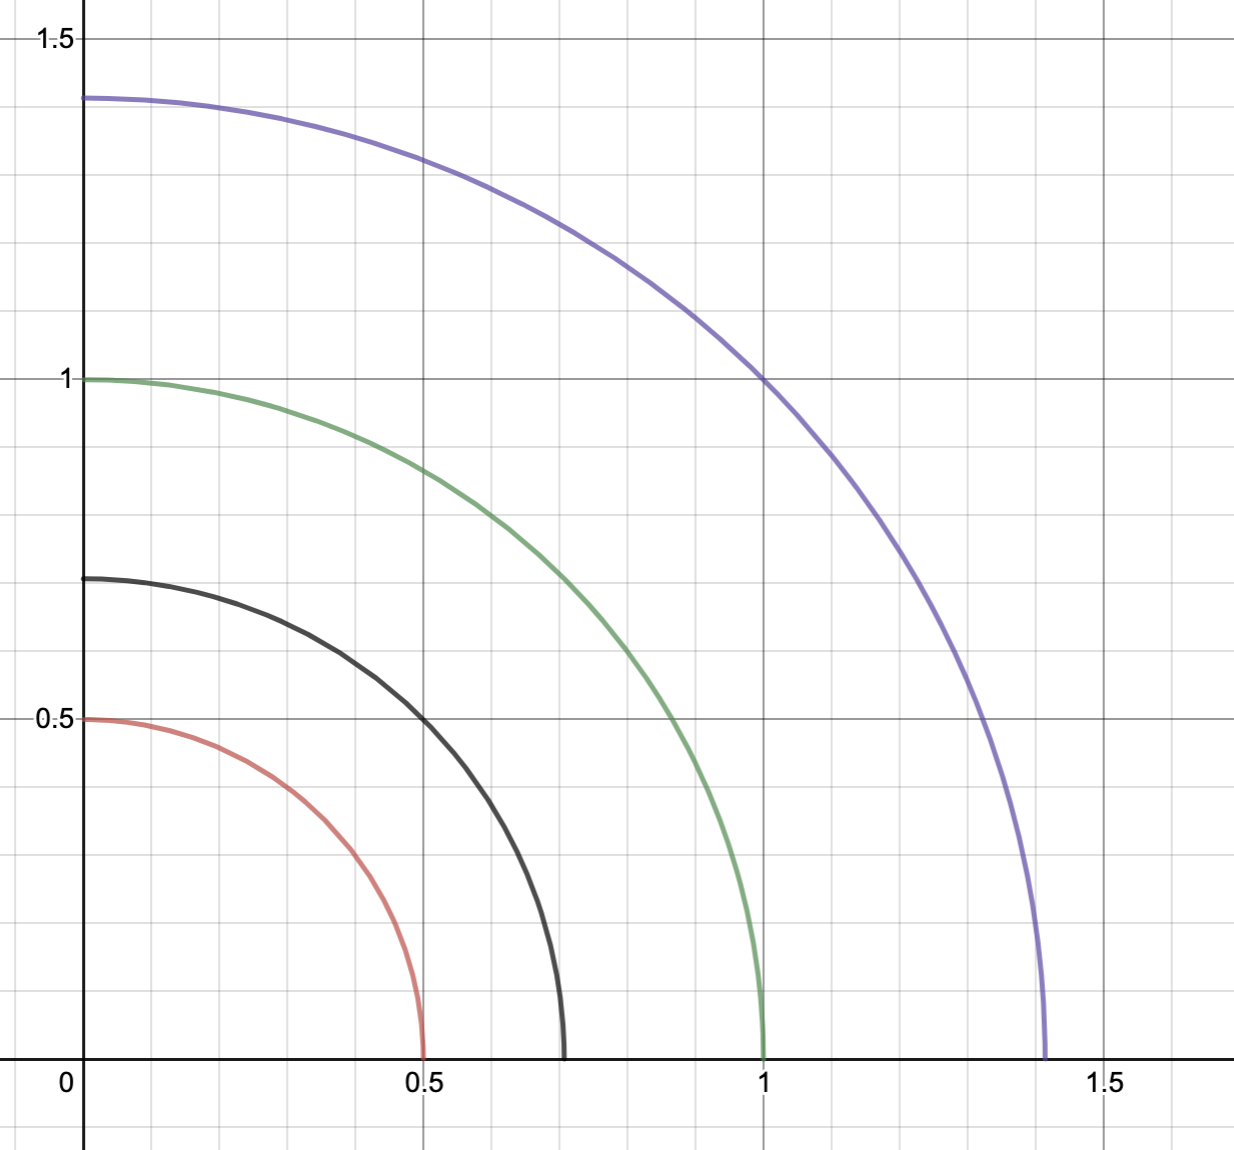
\includegraphics[scale=0.4]{concave_indiff}
\end{figure}

The issue with these indifference curves is that in any optimization problem under a budget constraint, the optimal bundles will be at the boundary points of the budget set (i.e. consuming only one good), and will not satisfy the typical first-order conditions.

The slope of the indifference curve is $-1$ times the marginal rate of substitution, or
\[ - \frac{\frac{\partial u}{\partial x_1}}{\frac{\partial u}{\partial x_2}} \]
In order for this to be convex, we need
 \[ - \frac{\partial}{\partial x_1} \frac{\frac{\partial u}{\partial x_1}}{\frac{\partial u}{\partial x_2}} > 0 \]
 Simplifying, we get
 \[ -  \frac{\frac{\partial u}{\partial x_2}\frac{\partial^2 u}{\partial x_1^2} - \frac{\partial u}{\partial x_1}\frac{\partial^2 u}{\partial x_1 \partial x_2}}{\left( \frac{\partial u}{\partial x_2} \right)^2} > 0 \]
 \[ \frac{\partial u}{\partial x_2}\frac{\partial^2 u}{\partial x_1^2} <  \frac{\partial u}{\partial x_1}\frac{\partial^2 u}{\partial x_1 \partial x_2} \]
 Note that this neither implies nor is implied by diminishing marginal utility.
\paragraph{(6.3)}
For the utility maximization, the second order conditions are that the determinant of the bordered Hessian is positive. For two goods, this implies that
\[ \det \left(\begin{bmatrix}
0 & -p_1 & -p_2 \\
-p_1 & \frac{\partial^2 u}{\partial x_1^2} & \frac{\partial^2 u }{\partial x_1 \partial x_2} \\
-p_2 & \frac{\partial^2 u}{\partial x_1 \partial x_2} & \frac{\partial^2 u}{\partial x_2^2} \\
\end{bmatrix} \right) > 0 \]
Diminishing marginal utility requires the diagonal entries to be negative, which is not necessary by the second order condition.
\paragraph{(6.4)}
Consider the Cobb-Douglas utility:
\[ u(x_1, x_2) = x_1^2x_2^2 \]
Then
\[ \frac{\partial^2 u}{\partial x_1^2} = 2x_2^2 \]
\[ \frac{\partial^2 u}{\partial x_2^2} = 2x_1^2 \]
which are both positive. However, the demand functions:
\[ x_1(p_1, p_2, w) = \frac{w}{2p_1} \]
\[ x_2(p_1, p_2, w) = \frac{w}{2p_2} \]
are downward sloping in $p_1, p_2$.
\paragraph{(6.5)}
The idea for diminishing marginal utility is to suggest convexity of the indifference curves, which is sufficient to satisfy the second-order conditions. However, decreasing marginal utility is not actually equivalent to convexity of the indifference curves, but in introductory economics classes that don't introduce a notion of the marginal rate of substitution, diminishing marginal utility is a misleading concept used instead.
\section*{Problem 7}
\paragraph{(7.1)}
Let's take a Cobb-Douglas utility. Let $x_1$ denote consumption of tobacco, and $x_2$ be the consumption of another good. Let the utility be
\[ u(x_1, x_2) = \alpha \log x_1 + (1-\alpha) \log x_2 \]
$\alpha$ parametrizes the strength of preference for tobacco. The Walrasian demand function for tobacco:
\[ x_1(p_1, p_2, w) = \frac{\alpha w}{p_1} \]
Note that in our case, the consumption of tobacco is linear in $\alpha$, hence as $\alpha$ decreases, so does tobacco consumption.
\paragraph{(7.2)}
Let $x_3$ denote the utility from health, so the utility function is now:
\[ u(x_1, x_2, x_3) = \alpha \log(x_1) + (1-\alpha) \log(x_2) + \log(x_3)  \]
Additionally, let's require the constraint $x_3 = H/x_1^\gamma$, $\gamma > 0$. This ensures that $x_1$ and $x_3$ are inversely related. Then we can rewrite the utility as
\[ u(x_1, x_2) =  \alpha \log(x_1) + (1-\alpha) \log(x_2) + \log(H/x_1) = (\alpha - \gamma) \log(x_1) + (1-\alpha) \log(x_2) + \log (H) \]
Once again, we assume $\alpha \in (0,1)$. The Walrasian demand for tobacco is given by
\[ x_1(p_1, p_2, w) = \frac{(\alpha - \gamma)w}{(1-\gamma)p_1} \]
The parameter $\gamma$ captures recognition that tobacco is bad for health. We have
\[ \frac{dx_1}{d\gamma} = \frac{w}{p_1}\frac{\alpha - 1}{(1-\gamma)^2}  \]
Note that since $\alpha < 1$, this expression is negative. Hence, as $\gamma$ increases, consumption of tobacco decreases.
\paragraph{(7.3)}
We would prefer to describe this as a change in constraint if we want to maintain assumptions about utility functions being invariant across time; a change in taste implies that the utility function has changed, whereas a change in constraint implies that the feasible set has changed. 

\end{document}
	% line of code telling latex that your document is ending. If you leave this out, you'll get an error
